\documentclass{tubaf-article}
\usepackage{graphicx}
\usepackage{subcaption}

\begin{document}
	\title{Scientific Computing Project}
	\subtitle{Winter Semester 2024/2025}
	\author{Lars Wunderlich \and Parsa Besharat \and Toni Sand}
	\date{April 6, 2025}
	\subject{Documentation}
	\publishers{TU Bergakademie Freiberg}
	
	\maketitle
	
	\tableofcontents
	
	\newpage
	
	\section{Task}
	
	The goal of this project was to code the model of a convolutional neural network and train it for the task of classifying images which consists of assigning them to one of 10 possible classes. The used training images are self-generated by the students of this course and collected into a database. A detailed description of the used training data can be found in chapter \ref{dataset}, whereas the architecture of the network is explained in chapter \ref{architecture}. Especially, the network should also be able to classify new images correctly. In chapter \ref{training} we talk about the training process and the tuning of hyperparameters like learning rate, batch size or optimizer by using k-fold cross-validation. At the end in chapter \ref{results}, we evaluate the result of our work by looking at several performance measurements like the confusion matrix and the loss and accuracy curves. Finally, we discuss approaches for improvement.
	
	\section{Description of the Data Set}
	\label{dataset}
	The data set that is used for the project consists of 10 classes of images. These are
	\begin{center}
		\begin{tabular}{ c c c c c }
			1. bottles & 2. mugs/cups & 3. spoons & 4. knifes & 5. forks \\ 
			6. shoes & 7. t-shirts & 8. plants & 9. chairs & 10. bikes    
		\end{tabular}
	\end{center}
	Every student had to contribute to this database by generating 15-20 pictures of pairwise disjoint objects for each class. In total there are approximately 400 images per class which yield a database of almost 4000 images. 
	\begin{figure}[h!]
		\centering
		% Erstes Bild
		\begin{subfigure}[b]{0.3\textwidth}
			\centering
			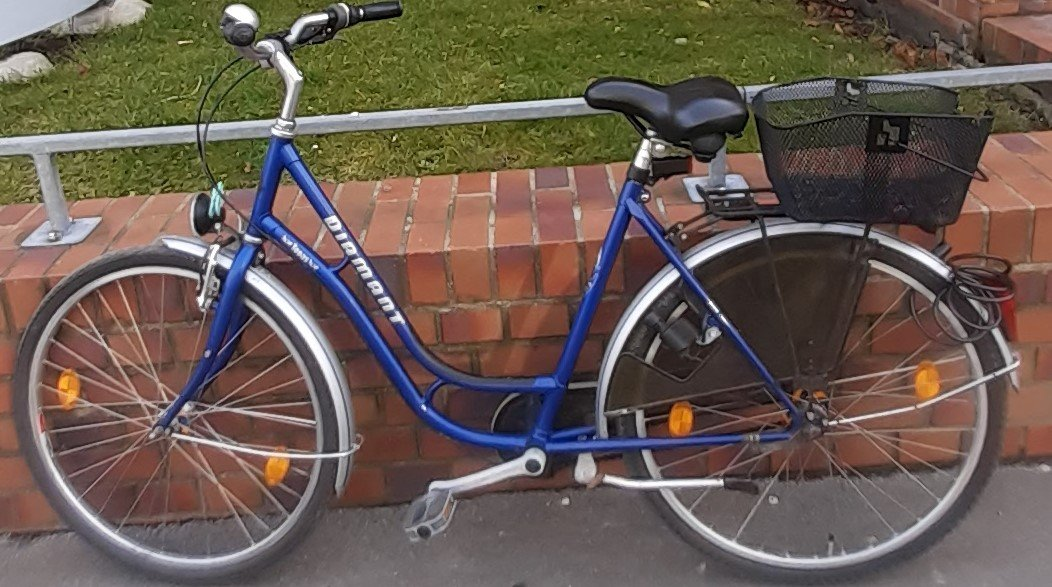
\includegraphics[width=\textwidth]{ex1.jpeg}
			\caption{10. bikes}
			\label{fig:bild1}
		\end{subfigure}
		\hfill
		% Zweites Bild
		\begin{subfigure}[b]{0.3\textwidth}
			\centering
			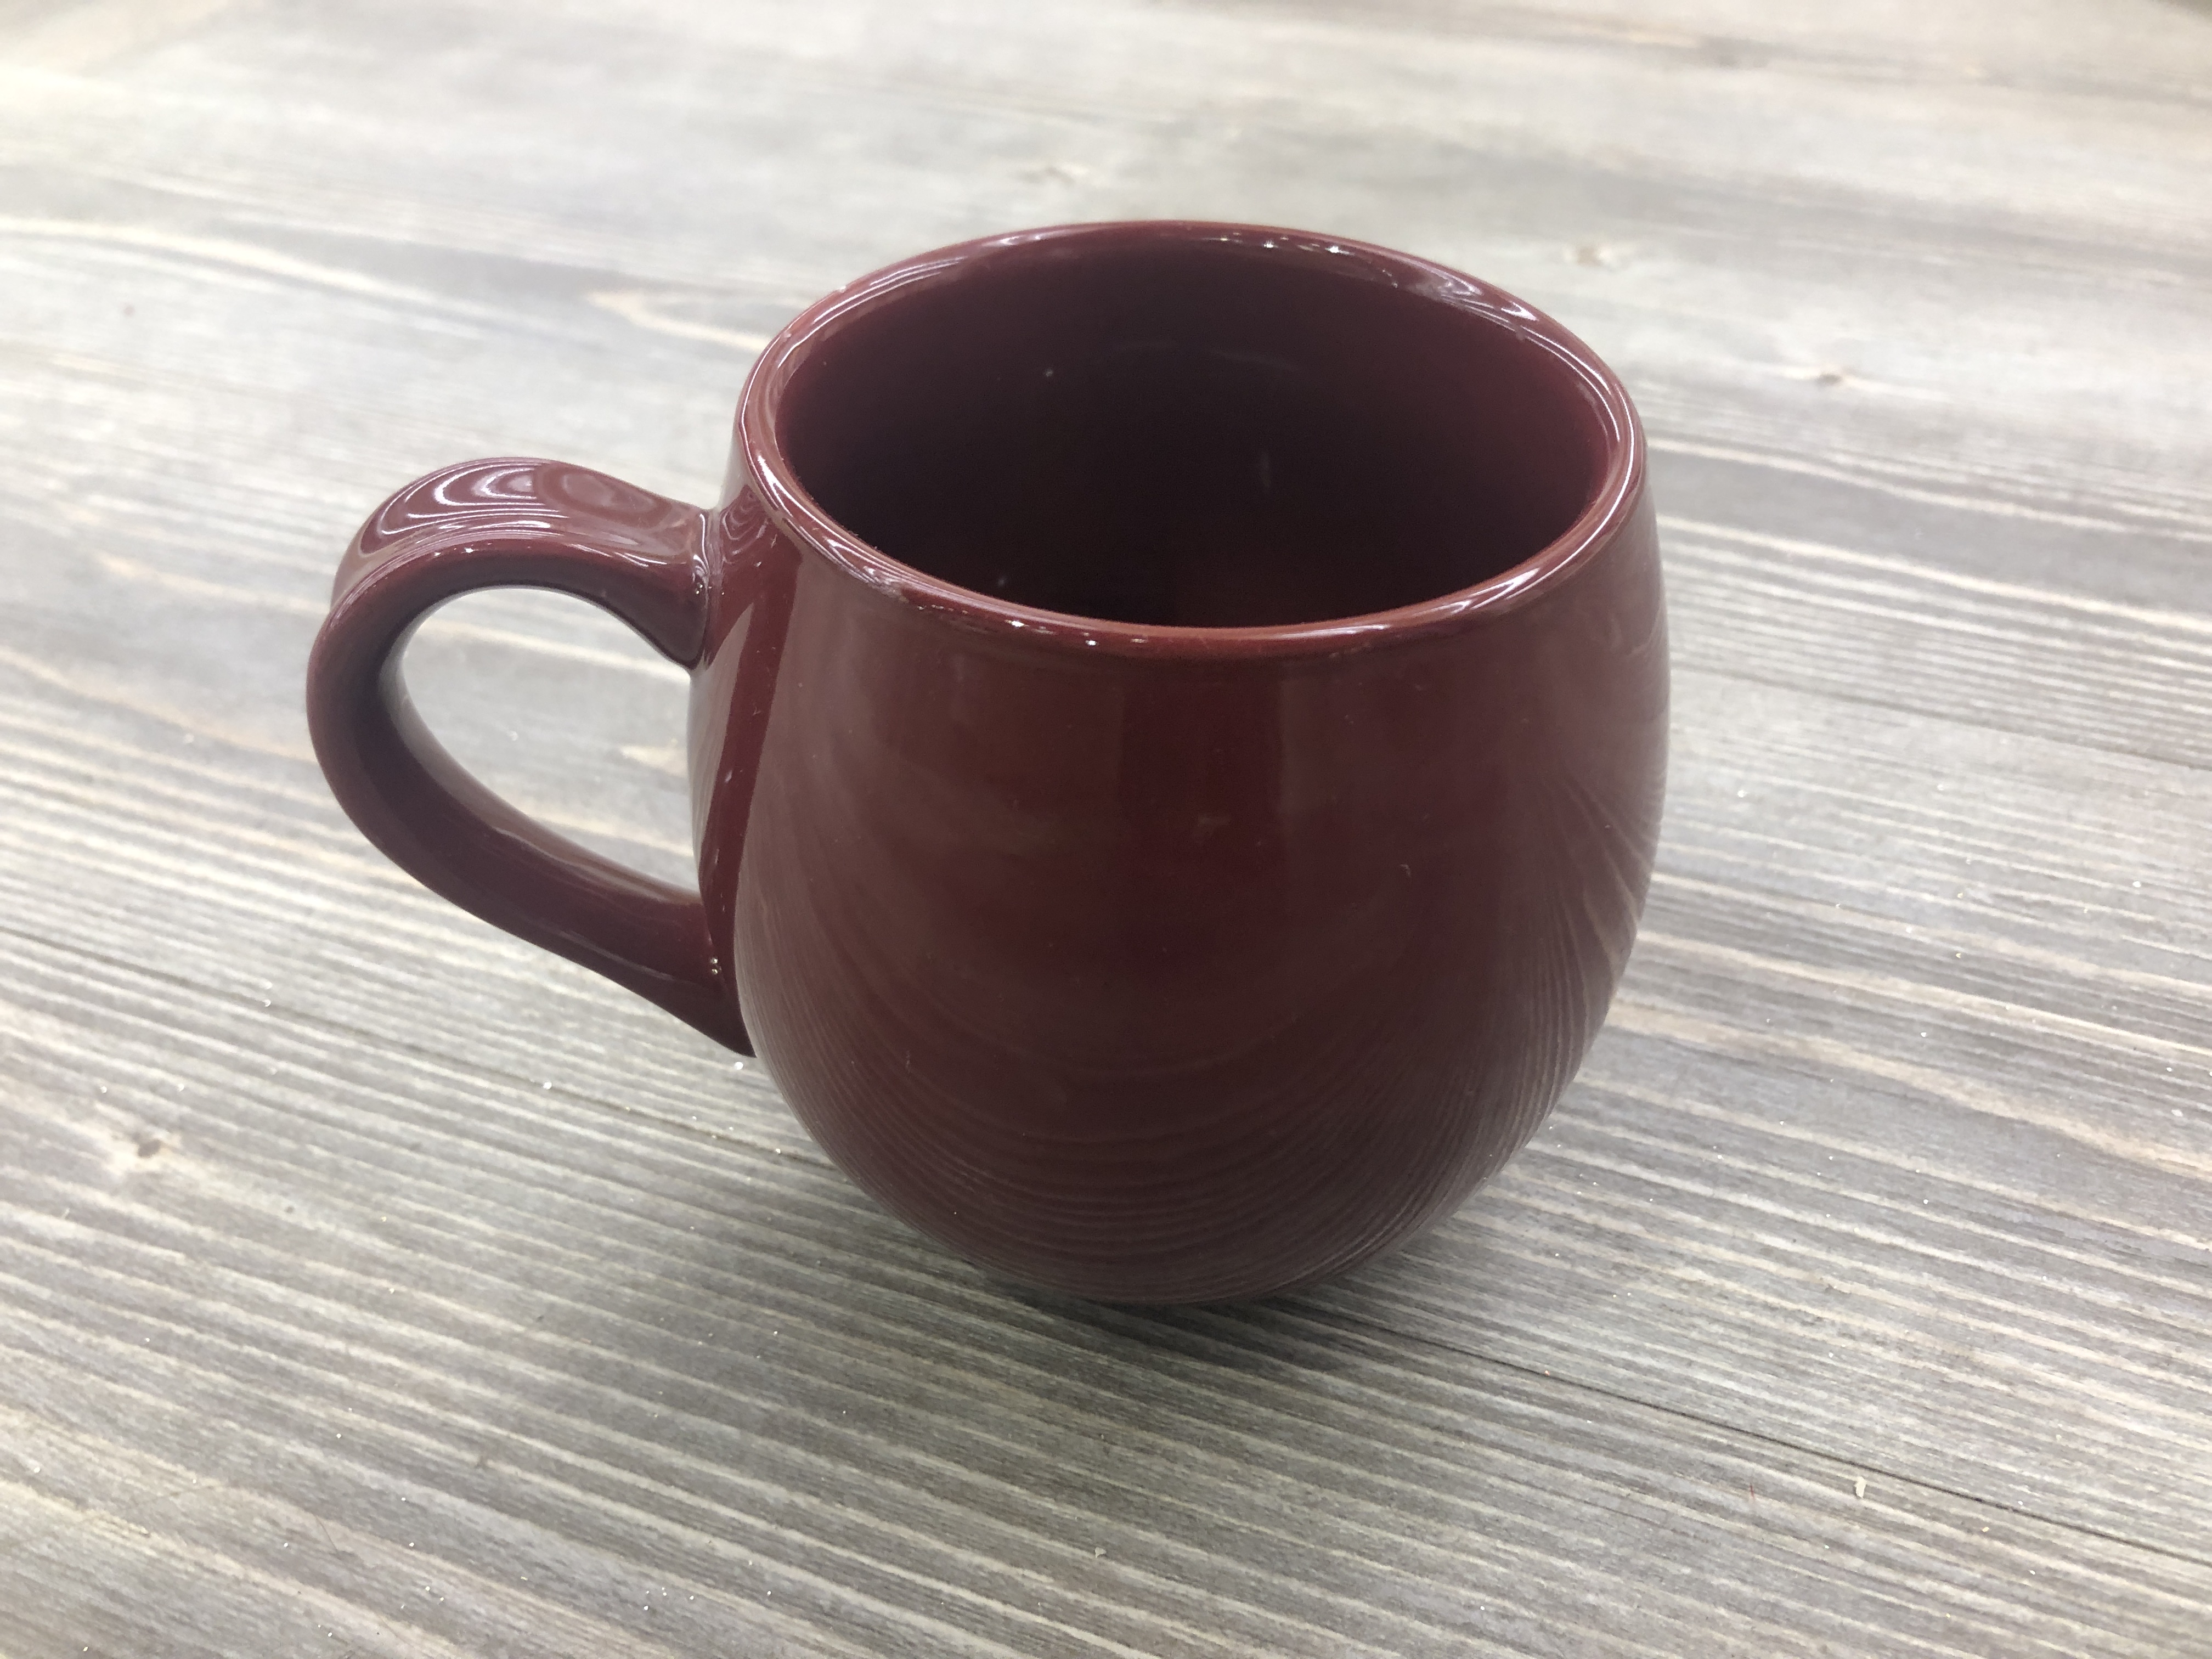
\includegraphics[width=\textwidth]{ex3.jpeg}
			\caption{2. mugs/cups}
			\label{fig:bild2}
		\end{subfigure}
		\hfill
		% Drittes Bild
		\begin{subfigure}[b]{0.3\textwidth}
			\centering
			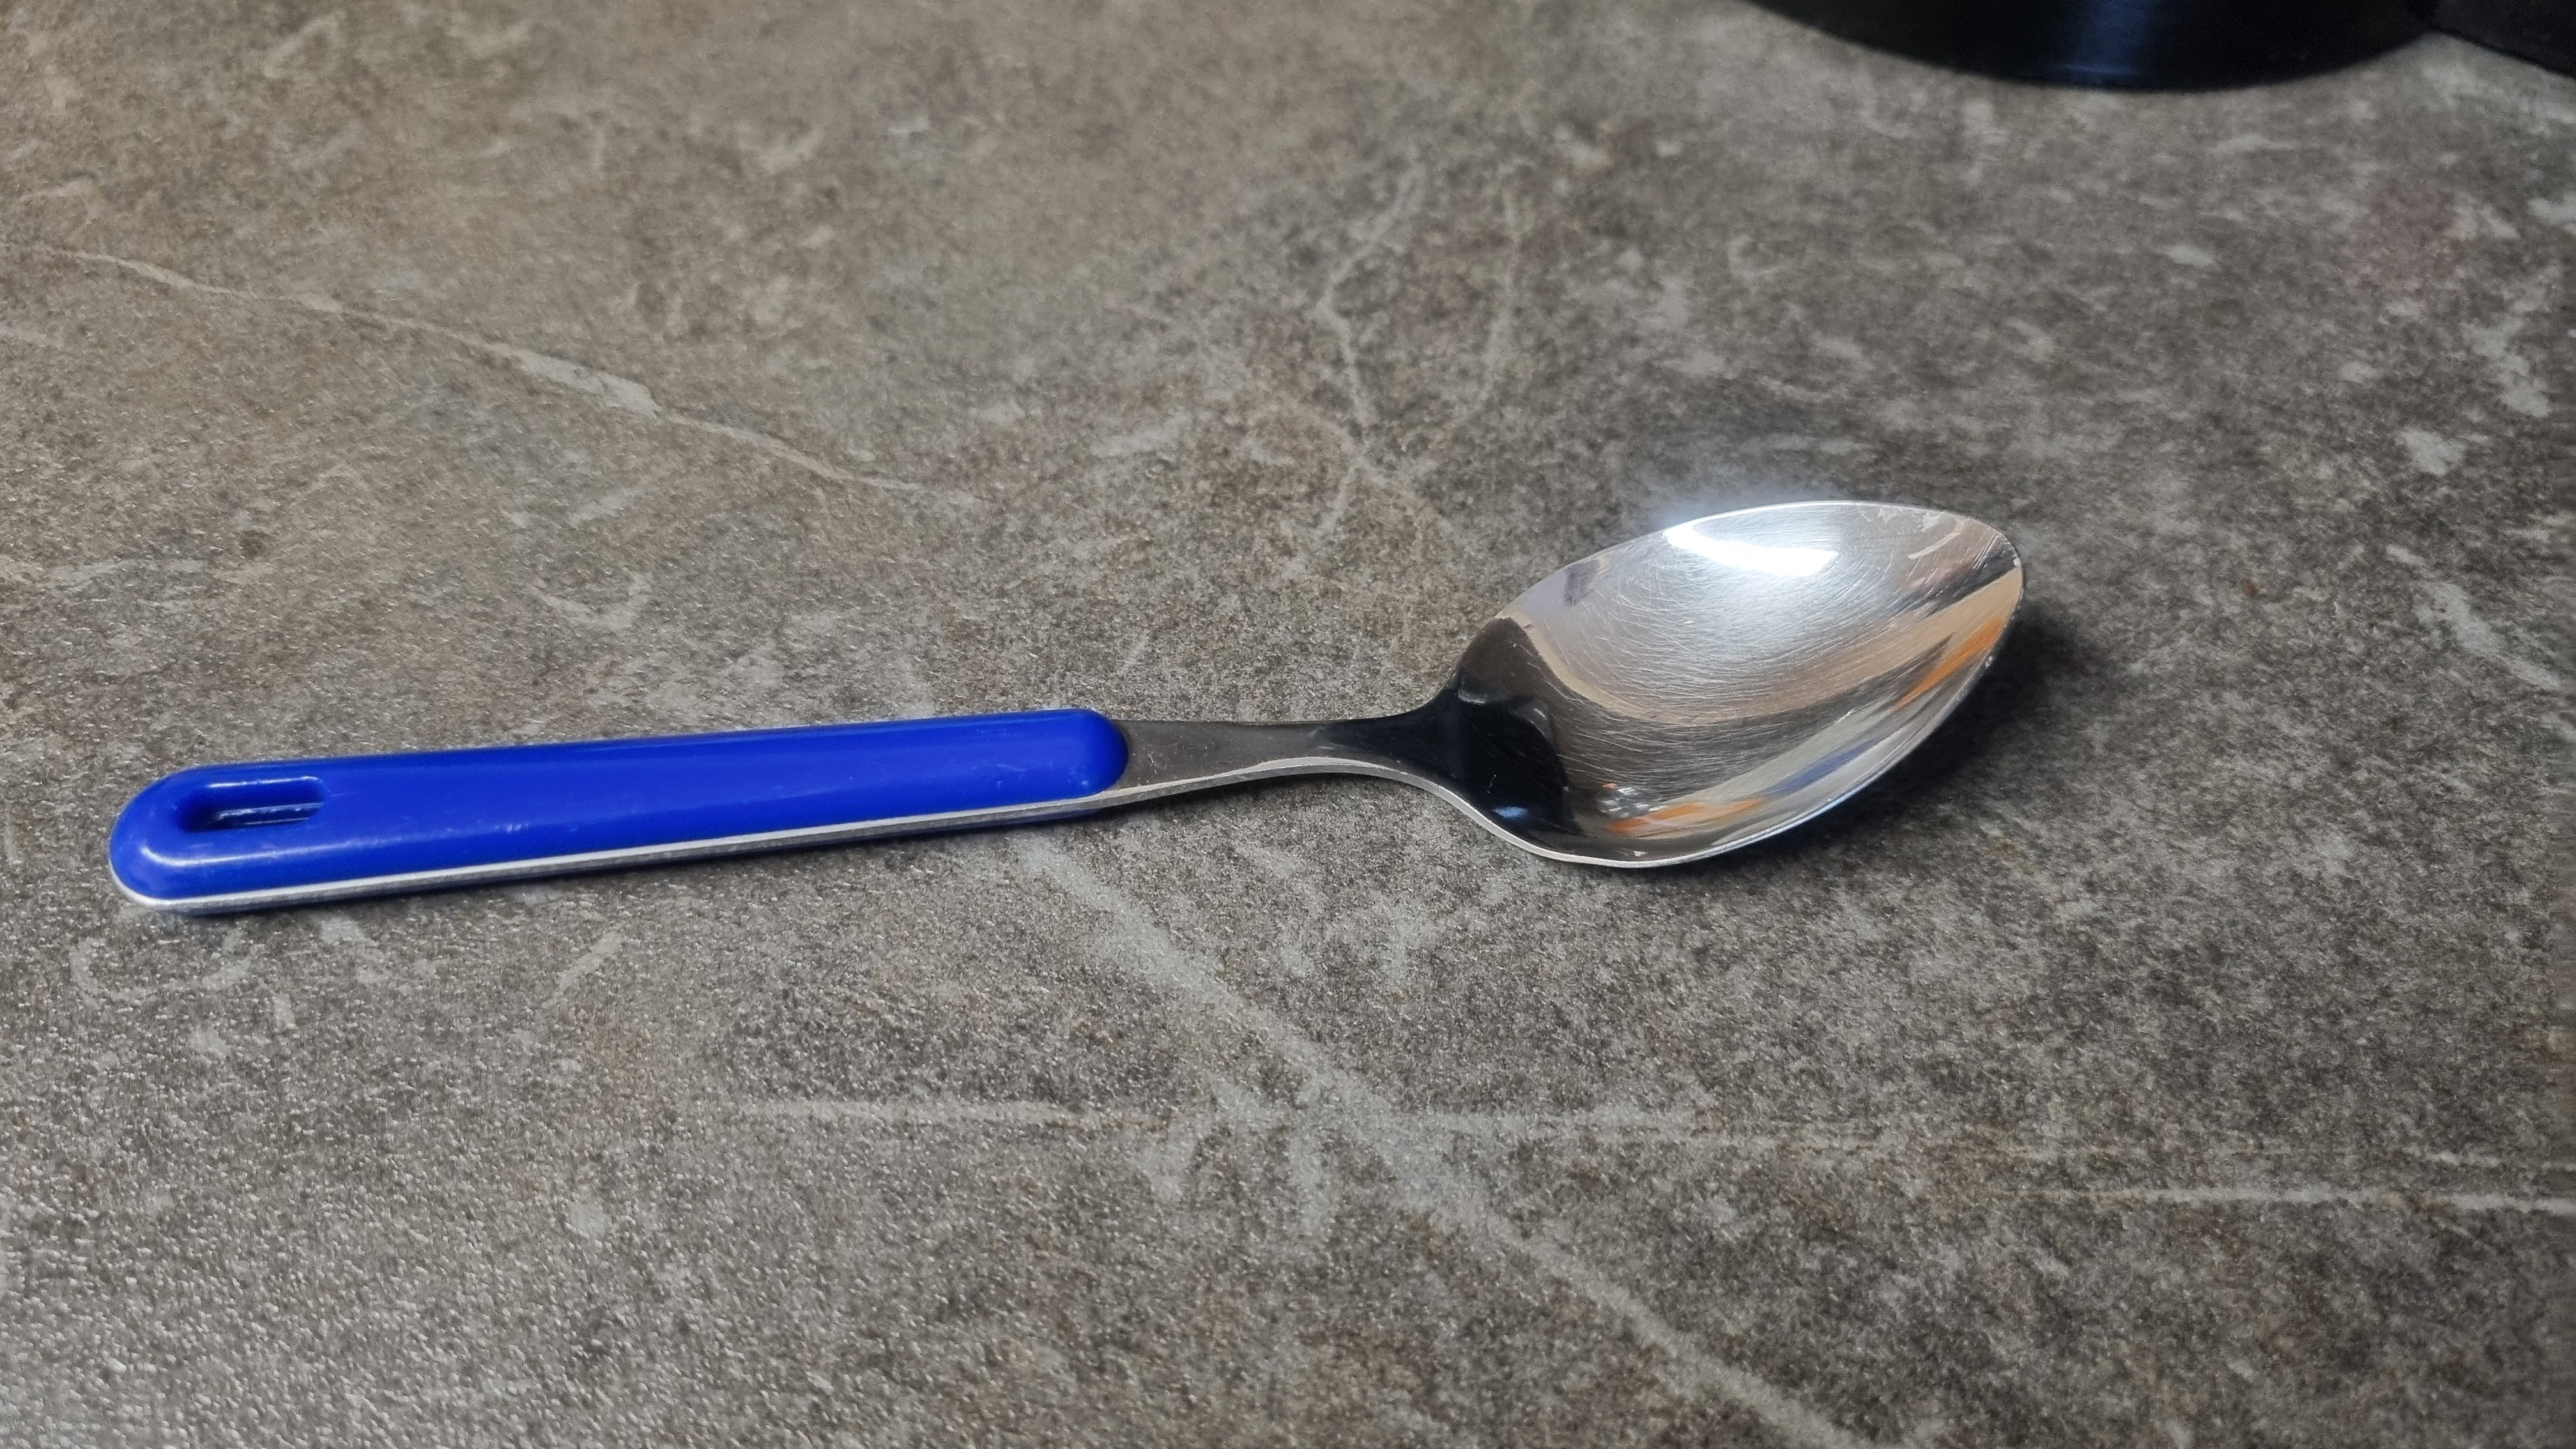
\includegraphics[width=\textwidth]{ex2.jpeg}
			\caption{3. spoons}
			\label{fig:bild2}
		\end{subfigure}
		\hfill
		\caption{Example images of some classes}
		\label{fig:nebeneinander}
	\end{figure}
	In the next step the images of the database were normalized to a resolution of 56x56 pixels. That made the training possible, despite the different resolutions in the beginning. To enlarge the database and improve the training process, we used the following augmentation techniques: \\
	\begin{itemize}
		\item horizontal flip
		\item vertical flip
		\item crop
		\item rotation 
		\item blur
		\item change of brightness
		\item change of contrast
		\item change of color
	\end{itemize}
	Here the intensity of the effects and attributes like the rotation angle are selected randomly based on a uniform distribution. It is also possible that more than one effect is applied simultaneously to one image. The number of these applied effects on this image is chosen randomly in the same manner but with a maximum of four. \\
	\textbf{TODO: insert example augmented images} \\
	As a result of this preprocessing procedure, we got 1500 images for every class and therefore a total database of around 15000 images for the training and testing of our neural network. 
	
	
	\section{Architecture of the Network}
	\label{architecture}
	For our convolutional neural network we were given the architecture of a simplified VGG-16 that we should implement. A VGG-16 is characterized by a very deep but uniform architecture, i.e. many convolutional layers in a row with a kernel size of 3, followed by a pooling layer. The simplified version of the VGG-16 uses fewer repetitions of these layers. In our case we used 4 repetitions after the initial convolutional layers with max pooling. \\
	\textbf{TODO: insert picture of the architecture} \\
	The first convolutional layer gets the 56x56 image with the 3 color channels as input and convolutes it to 64 channels while preserving the resolution because of the kernel size of 3 and the padding of 1. After that another convolutional layer is applied again preserving both resolution and number of channels. The following max pooling halfes the image resolution to 28x28 due to the kernel size and stride of 2. This procedure is repeated with again 2 convolutional layers and a max pooling that halfes the image resolution and doubles the number of channels in the end. After this, there are 3 more repetitions acting in a similar manner but with 3 convolutional layers instead of 2. Subsequently 4 fully connected layers are applied. The reason for choosing such a high number of channels is to enable the network to learn the high variety of features in the complex input images and focus less on the spatial resolution. In the whole network ReLU is used as activation function. Furthermore we applied a batch normalization to the output of every convolutional layer so that the training process behaves more stable by fixing the means and variances of each layers inputs. This helps speeding up the training and improves the generalization properties, i.e. reducing overfitting.
	
	
	\section{Training}
	\label{training}
	
	
	
	\section{Results}
	\label{results}
	
\end{document}
